%% The PHY design logic, as the code actually runs it
%% (drivers/usrp/include/physical_layer.hpp + ACQ_stop_and_wait.hpp).
%% Geometry: a U. Transmit chain left-to-right along the top, the air closes
%% the RIGHT side, receive chain flows back along the bottom rows, and the ACK
%% closes the LEFT side. Every connector has its own lane (x=-13, x=5W+8,
%% y=-49), so nothing crosses a box. Colours say which layer owns a stage.
\documentclass[tikz,border=4pt]{standalone}
\usepackage{xcolor}
%% Shared look for the UnionLabs system figures. \input by each fig-*.tex so a
%% colour or a corner radius is changed in one place.
\usetikzlibrary{positioning,arrows.meta,fit,backgrounds,calc}

\definecolor{uCode}{HTML}{1F6F5C}     % the experimenter's own code
\definecolor{uApi}{HTML}{6B4BA8}      % the contract / ARQ layer
\definecolor{uPhy}{HTML}{2E5E9E}      % transports / DSP
\definecolor{uRadio}{HTML}{B4700F}    % hardware
\definecolor{uShare}{HTML}{8A2E4D}    % the shared workspace

\tikzset{
  blk/.style={draw, rounded corners=2pt, align=center, font=\small,
              minimum height=8mm, inner sep=3pt, fill=black!2},
  code/.style={blk, draw=uCode, thick, fill=uCode!6},
  api/.style={blk, draw=uApi, very thick, fill=uApi!7},
  phy/.style={blk, draw=uPhy, thick, fill=uPhy!6},
  radio/.style={blk, draw=uRadio, thick, fill=uRadio!8},
  share/.style={blk, draw=uShare, thick, fill=uShare!6},
  stage/.style={blk, minimum height=9.5mm, font=\scriptsize, text width=16mm,
                inner sep=2pt},
  flow/.style={-{Latex[length=2mm]}, thick},
  back/.style={-{Latex[length=2mm]}, thick, densely dashed},
  % labels that sit ON an arrow: opaque, so the line never strikes the text
  onarrow/.style={font=\scriptsize\itshape, fill=white, inner sep=1.5pt},
  lbl/.style={font=\scriptsize\itshape, inner sep=1pt},
  note/.style={font=\scriptsize, align=left, inner sep=1pt},
  legend/.style={draw, minimum width=3mm, minimum height=3mm, inner sep=0pt},
}
\newcommand{\mono}[1]{{\ttfamily\footnotesize #1}}
\newcommand{\monos}[1]{{\ttfamily\scriptsize #1}}

\begin{document}
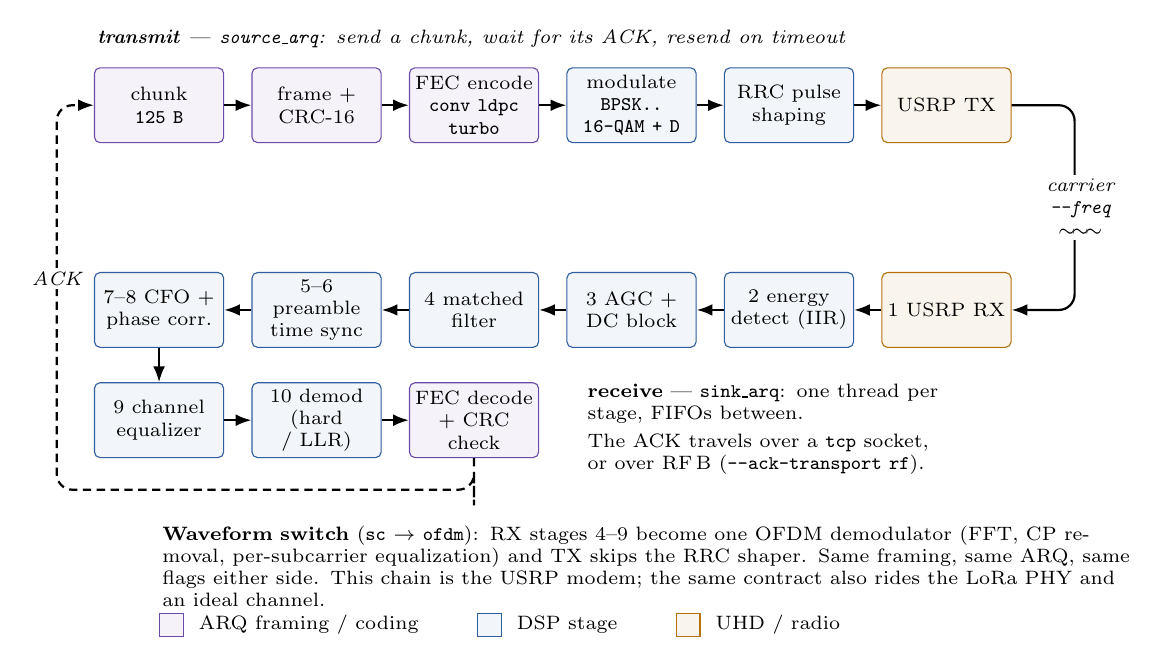
\begin{tikzpicture}[x=1mm, y=1mm,
  stage/.append style={text width=15mm}]

\def\W{20}   % column pitch (boxes ~17mm wide -> ~3mm gap between columns)

%% ── TX row, left to right ─────────────────────────────────────────────────
\node[stage, fill=uApi!7,  draw=uApi]  (chunk) at (0,0)    {chunk\\\monos{125 B}};
\node[stage, fill=uApi!7,  draw=uApi]  (crc)   at (\W,0)   {frame +\\CRC-16};
\node[stage, fill=uApi!7,  draw=uApi]  (fec)   at (2*\W,0) {FEC encode\\\monos{conv ldpc}\\\monos{turbo}};
\node[stage, fill=uPhy!6,  draw=uPhy]  (mod)   at (3*\W,0) {modulate\\\monos{BPSK..}\\\monos{16-QAM + D}};
\node[stage, fill=uPhy!6,  draw=uPhy]  (rrc)   at (4*\W,0) {RRC pulse\\shaping};
\node[stage, fill=uRadio!8,draw=uRadio](tx)    at (5*\W,0) {USRP TX};
\node[lbl, above=2mm of chunk.north west, anchor=south west]
  {\textbf{transmit} --- \monos{source\_arq}: send a chunk, wait for its ACK, resend on timeout};

\draw[flow] (chunk) -- (crc);
\draw[flow] (crc) -- (fec);
\draw[flow] (fec) -- (mod);
\draw[flow] (mod) -- (rrc);
\draw[flow] (rrc) -- (tx);

%% ── RX rows: back along the bottom, numbered as the threads launch ────────
\node[stage, fill=uRadio!8,draw=uRadio](rx)  at (5*\W,-26) {1 USRP RX};
\node[stage, fill=uPhy!6, draw=uPhy] (det)   at (4*\W,-26) {2 energy\\detect (IIR)};
\node[stage, fill=uPhy!6, draw=uPhy] (agc)   at (3*\W,-26) {3 AGC +\\DC block};
\node[stage, fill=uPhy!6, draw=uPhy] (mf)    at (2*\W,-26) {4 matched\\filter};
\node[stage, fill=uPhy!6, draw=uPhy] (sync)  at (\W,-26)   {5--6 preamble\\time sync};
\node[stage, fill=uPhy!6, draw=uPhy] (cfo)   at (0,-26)    {7--8 CFO +\\phase corr.};
\node[stage, fill=uPhy!6, draw=uPhy] (eq)    at (0,-40)    {9 channel\\equalizer};
\node[stage, fill=uPhy!6, draw=uPhy] (dem)   at (\W,-40)   {10 demod\\(hard / LLR)};
\node[stage, fill=uApi!7, draw=uApi] (dec)   at (2*\W,-40) {FEC decode\\+ CRC check};

%% ── the air closes the right side ─────────────────────────────────────────
\draw[flow, rounded corners=2mm] (tx.east) -- ++(8,0) |- (rx.east);
\node[onarrow, align=center] at (5*\W+17,-13)
  {carrier\\\monos{--freq}\\$\sim\!\sim\!\sim$};

\draw[flow] (rx) -- (det);
\draw[flow] (det) -- (agc);
\draw[flow] (agc) -- (mf);
\draw[flow] (mf) -- (sync);
\draw[flow] (sync) -- (cfo);
\draw[flow] (cfo) -- (eq);
\draw[flow] (eq) -- (dem);
\draw[flow] (dem) -- (dec);

%% ── the ACK closes the left side: down, along y=-49, up x=-13 ────────────
\draw[back, rounded corners=2mm]
  (dec.south) -- ++(0,-4) -- ++(0,-0.01) -| (-13,0) -- (chunk.west);
\node[onarrow] at (-13,-22) {ACK};

%% ── receive + ACK-transport note, in the empty right-bottom region ───────
\node[note, anchor=north west, text width=52mm] at (2*\W+14,-35)
  {\textbf{receive} --- \monos{sink\_arq}: one thread per\\ stage, FIFOs between.\\[2pt]
   The ACK travels over a \monos{tcp} socket,\\ or over RF\,B
   (\monos{--ack-transport rf}).};

%% ── waveform switch, then the legend, stacked clear of everything ────────
\node[note, text width=124mm, anchor=north west] (wnote) at (0,-53)
  {\textbf{Waveform switch} (\monos{sc} $\rightarrow$ \monos{ofdm}): RX stages
   4--9 become one OFDM demodulator (FFT, CP removal, per-subcarrier
   equalization) and TX skips the RRC shaper. Same framing, same ARQ, same
   flags either side. This chain is the USRP modem; the same contract also
   rides the LoRa PHY and an ideal channel.};

\node[legend, draw=uApi, fill=uApi!7, anchor=west] (l1) at (0,-66) {};
\node[note, right=1.5mm of l1] (l1t) {ARQ framing / coding};
\node[legend, draw=uPhy, fill=uPhy!6, right=7mm of l1t] (l2) {};
\node[note, right=1.5mm of l2] (l2t) {DSP stage};
\node[legend, draw=uRadio, fill=uRadio!8, right=7mm of l2t] (l3) {};
\node[note, right=1.5mm of l3] {UHD / radio};

\end{tikzpicture}
\end{document}
